\documentclass[11pt, oneside]{article} 
\usepackage{geometry}
\geometry{letterpaper} 
\usepackage{graphicx}
	
\usepackage{amssymb}
\usepackage{amsmath}
\usepackage{parskip}
\usepackage{color}
\usepackage{hyperref}

\graphicspath{{/Users/telliott_admin/Dropbox/Tex/png/}}
% \begin{center} 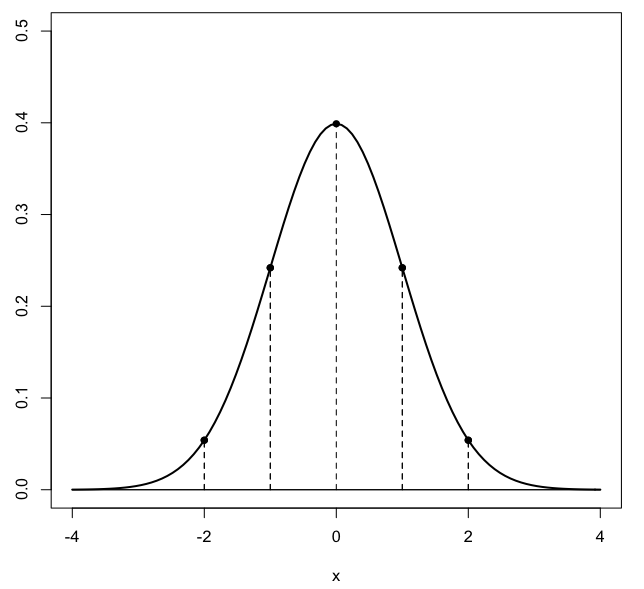
\includegraphics [scale=0.4] {gauss3.png} \end{center}

\title{Area}
\date{}

\begin{document}
\maketitle
\Large

One aspect of calculus will be to determine the area of figures in the plane, particularly figures bounded by curves, as well as volumes in space.  This is the magic of calculus, that we can make curves conform to rectilinear concepts of area and volume.

Since this introductory section is about Euclidean geometry, let's just say a few words about the area of a triangle.  But we'll start with the rectangle.

To find the area of a rectangle, we must first fix a unit length.  Then multiply the width by the height.
\begin{center} 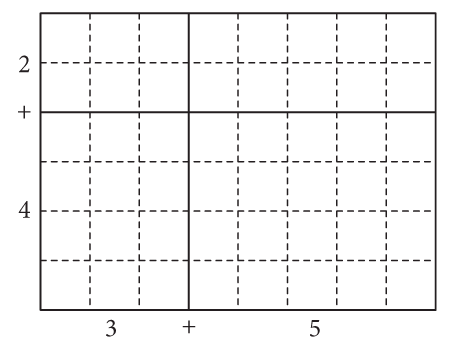
\includegraphics [scale=0.3] {area5.png} \end{center}
This particular figure (from Lockhart) shows the distributive law in action:
\[ (3 + 5) \cdot (4 + 2) \]
\[ =3 \cdot 4 + 3 \cdot 2 + 5 \cdot 4 + 5 \cdot 2 \]
\[ = 48 \]
Any combination of numbers that add up to $8$, times any combination of numbers that add up to $6$, gives the same result.

The next figure is a parallelogram, a four-sided figure whose two pairs opposite sides are parallel (left panel).  As a consequence of the theorems we saw previously, the opposing angles are equal, and the adjacent angles add up to 180 degrees.
\begin{center} 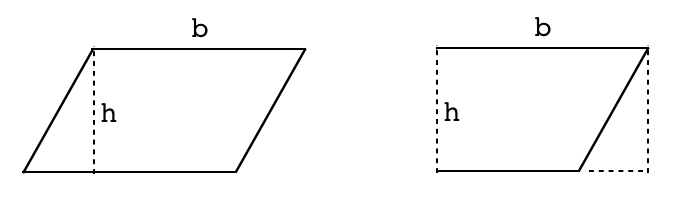
\includegraphics [scale=0.4] {area7.png} \end{center}
To find the area, we cut off a right triangle from the left and re-attach it on the right.  The angles add up to form a straight line along the base and a right triangle at the upper right.    The area is clearly $h \times b$.

What about triangles?  Well, every triangle can be turned into a parallelogram, by attaching a rotated image of itself, like this:
\begin{center} 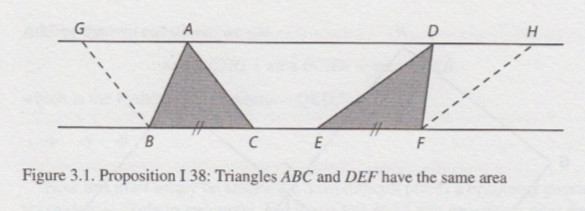
\includegraphics [scale=0.6] {area6.png} \end{center}

An acute triangle is on the left and an obtuse triangle on the right.  Since the area of each triangle is one-half that of its corresponding parallelogram (because we added the same area to make the parallelogram), the area of a triangle is one-half the base times the height.

\begin{center} 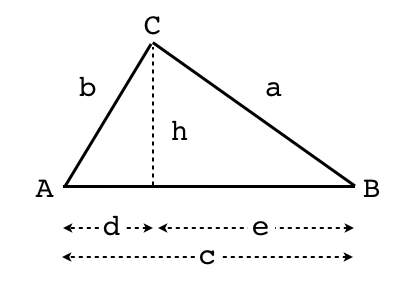
\includegraphics [scale=0.5] {Triangle.png} \end{center}

Here, the area is $hc/2$.

We could choose any side of the triangle to be the base and then multiply $1/2 \ \times$ base $\times$ height to get the area.  We must always get the same answer!

If you accept the argument about the parallelogram above, it must be true, because the area of the triangle has to be the same no matter how you calculate it.  Here's a proof:
\begin{center} 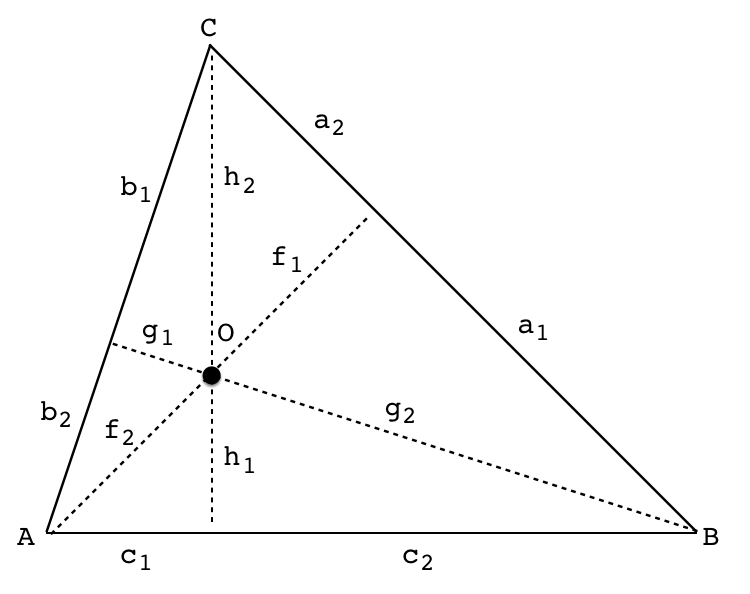
\includegraphics [scale=0.3] {area8.png} \end{center}
In $\triangle ABC$ with sides $a,b,c$, drop the three altitudes from each of the three vertices to form right angles on the opposing sides.  Ceva's theorem says that these altitudes cross at a single point (we will prove this later).  Label the parts of the sides and the altitudes as shown in the diagram.

The area of the whole $\triangle ABC$ is equal to the sum
\[ \triangle BOC + \triangle AOC + \triangle AOB \]
Using the rule, \emph{twice} the area is
\[ 2A = af_1 + bg_1 + ch_1 \]

But each of these smaller areas can be computed in different ways.  In particular $\triangle BOC$ can be viewed as having base $g_2$ and height $b_1$, while $\triangle AOB$ can be viewed as having base $b_2$ and height $g_2$, so (twice) the total area is also
\[ 2A = b_1 g_2 + b_2 g_2 + b g_1 \]
\[ = b g_2 + b g_1 = bg \]

Similar calculations can be carried out for the other two sides.  Hence the area is the same regardless of which side is chosen as the base.

$\square$

A corollary is that all triangles with the same base and height have the same area.
\begin{center} 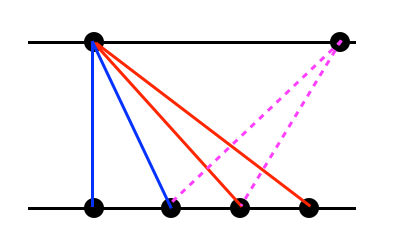
\includegraphics [scale=0.5] {triangles_parallel.png} \end{center}

\end{document}